% Created 2023-03-30 Thu 15:38
% Intended LaTeX compiler: lualatex
\documentclass[11pt]{article}
\usepackage[margin=0.5in]{geometry}
\usepackage{syntax}
\usepackage{pdfpages}
\usepackage{tcolorbox}
\usepackage{etoolbox}
\usepackage{environ}
\usepackage[ruled]{algorithm2e}
\let\oldtabular\tabular
\let\oldendtabular\endtabular
\NewEnviron{tabular2}[1]{\tcbox[left=0mm, right=0mm, top=0mm, bottom=0mm]{\oldtabular{#1}\BODY\oldendtabular}}
\BeforeBeginEnvironment{minted}{\begin{tcolorbox}}%
\AfterEndEnvironment{minted}{\end{tcolorbox}}
\BeforeBeginEnvironment{verbatim}{\begin{tcolorbox}}%
\AfterEndEnvironment{verbatim}{\end{tcolorbox}}
\usepackage{graphicx}
\usepackage{longtable}
\usepackage{wrapfig}
\usepackage{rotating}
\usepackage[normalem]{ulem}
\usepackage{amsmath}
\usepackage{amssymb}
\usepackage{capt-of}
\usepackage{hyperref}
\usepackage{minted}
\usepackage{physics}
\author{David Lewis}
\date{}
\title{lecture 22}
\hypersetup{
 pdfauthor={David Lewis},
 pdftitle={lecture 22},
 pdfkeywords={},
 pdfsubject={},
 pdfcreator={Emacs 30.0.50 (Org mode 9.6.1)}, 
 pdflang={English}}
\begin{document}

\maketitle
\section*{1.}
\label{sec:org94fde8f}
\begin{minted}[fontsize=\scriptsize]{python}
from math import sqrt
import numpy as np

D = {"A":[sqrt(2), sqrt(3), sqrt(5), 0, 0, 0],
     "B":[sqrt(2), 0, sqrt(5), 0, sqrt(6), 0],
     "C":[sqrt(2), 0, sqrt(5), 1, sqrt(6), 0],
     "D":[0, 0, 0, 0, sqrt(6), 2],
     "E":[0, 0, 0, 1, 0, 2]}
affinity = np.zeros((5, 5))
for xi in range(len(D)):
    for xj in range(len(D)):
        xivec = D[list(D.keys())[xi]]
        xjvec = D[list(D.keys())[xj]]
        affinity[xi, xj] = round(np.dot(np.array(xivec), np.array(xjvec)))
affinity.tolist()
\end{minted}
\begin{center}
\begin{tabular2}{rrrrr}
10.0 & 7.0 & 7.0 & 0.0 & 0.0\\[0pt]
7.0 & 13.0 & 13.0 & 6.0 & 0.0\\[0pt]
7.0 & 13.0 & 14.0 & 6.0 & 1.0\\[0pt]
0.0 & 6.0 & 6.0 & 10.0 & 4.0\\[0pt]
0.0 & 0.0 & 1.0 & 4.0 & 5.0\\[0pt]
\end{tabular2}
\end{center}

\begin{minted}[fontsize=\scriptsize]{python}
import networkx as nx
import matplotlib.pyplot as plt

G = nx.Graph()
G.add_nodes_from(list(D.keys()))

for i in range(len(D.keys())):
    for j in range(i+1, len(D.keys())):
        i_node = list(D.keys())[i]
        j_node = list(D.keys())[j]
        G.add_edge(i_node, j_node, weight=affinity[i, j])
ax_1 = plt.subplot(111)
pos=nx.spring_layout(G, seed=0)
nx.draw_networkx(G, pos, with_labels=True)
for edge in G.edges(data="weight"):
    nx.draw_networkx_edges(G, pos, edgelist=[edge], width=edge[2])
plt.show()

\end{minted}

\begin{center}
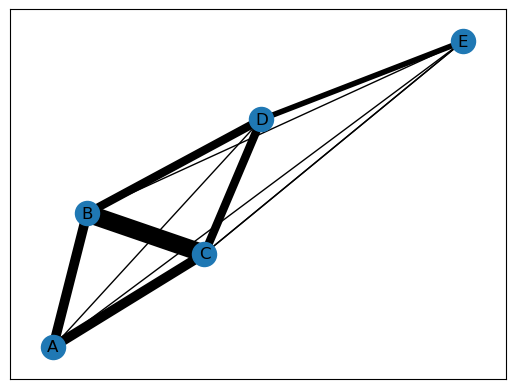
\includegraphics[width=0.7\textwidth]{./.ob-jupyter/b9ae460d0829f20394bc4a381df69a095b43ed4b.png}
\end{center}

It looks like ABCD are in one cluster and E is in another cluster.
\section*{2.}
\label{sec:org570cf3a}
\subsection*{a.}
\label{sec:orgfc64e8a}
\begin{itemize}
\item compute affinity matrix A
\item Set L = A
\item compute k(number of clusters) largest eigenvalues/eigenvectors of L
\item compute matrix Y from eigenvalue matrix U using \(y_i =
  \frac{1}{\sqrt{\sum^k_{j=1}u^2_{n-j+1, i}}}(\vec{u_i}^T)\)
\item find clusters using k-means on Y
\end{itemize}
\subsection*{b.}
\label{sec:org257de71}
\begin{minted}[fontsize=\scriptsize]{python}
import scipy
A = affinity
k = 2
L = A
eigenvalues, eigenvectors = scipy.linalg.eigh(L)
U = eigenvectors[:,[-k, -1]]
row_sums = np.sqrt(np.square(U).sum(axis=1, keepdims=True))

Y = U / row_sums
Centroids, euclidian_mean = scipy.cluster.vq.kmeans(Y, k)
Clusters, distances = scipy.cluster.vq.vq(Y, Centroids)
list(zip(Y.tolist(),Clusters))
\end{minted}


\begin{center}
\begin{tabular2}{lr}
Eigen Point & cluster\\[0pt]
\hline
(0.8252524486793774 -0.5647640179302249) & 0\\[0pt]
(0.12086906435542212 -0.9926684588934237) & 0\\[0pt]
(0.06222575627649513 -0.9980620998995093) & 0\\[0pt]
(-0.9131796757110512 -0.40755721054627325) & 1\\[0pt]
(-0.9887063042057109 -0.1498660869706164) & 1\\[0pt]
\end{tabular2}
\end{center}
\subsection*{c.}
\label{sec:orgab8ca52}
\begin{itemize}
\item compute affinity matrix
\item Compute Degree matrix
\begin{itemize}
\item diagonal matrix
\item each entry is the sum of weights of all edges incident with node
\end{itemize}
\item Compute L
\begin{itemize}
\item L = D - W
\end{itemize}
\item compute k(number of clusters) smallest eigenvalues/eigenvectors of L
\item compute matrix Y from eigenvalue matrix U using \(y_i =
  \frac{1}{\sqrt{\sum^k_{j=1}u^2_{n-j+1, i}}}(\vec{u_i}^T)\)
\item find clusters using k-means on Y
\end{itemize}
\subsection*{d.}
\label{sec:orgd0ea304}
\begin{minted}[fontsize=\scriptsize]{python}
import scipy
A = affinity
k = 2
# network x does weighted degrees for us!
D = np.diag(list(dict(G.degree(weight="weight")).values()))
L = D-A

eigenvalues, eigenvectors = scipy.linalg.eigh(L)
U = eigenvectors[:,:2]
row_sums = np.sqrt(np.square(U).sum(axis=1, keepdims=True))

Y = U / row_sums
Centroids, euclidian_mean = scipy.cluster.vq.kmeans(Y, k)
Clusters, distances = scipy.cluster.vq.vq(Y, Centroids)
list(zip(Y.tolist(),Clusters))
\end{minted}

\begin{center}
\begin{tabular2}{lr}
Eigen Point & cluster\\[0pt]
\hline
(-0.8264994349350939 -0.5629375489803203) & 1\\[0pt]
(-0.9670898580131041 -0.25443507330593085) & 1\\[0pt]
(-0.9806921960094918 -0.19555770679285542) & 1\\[0pt]
(-0.8201574486531152 0.5721378849707581) & 0\\[0pt]
(-0.21393030744777544 0.9768489256560097) & 0\\[0pt]
\end{tabular2}
\end{center}
\subsection*{e.}
\label{sec:orgae915f1}
The only difference is that L is computed either like L\textsuperscript{a} = D\textsuperscript{-1} L or like L\textsuperscript{s} =
D\textsuperscript{-.5} L D\textsuperscript{-.5}. We'll do both.

\begin{minted}[fontsize=\scriptsize]{python}
import scipy
A = affinity
k = 2
# network x does weighted degrees for us!
D = np.diag(list(dict(G.degree(weight="weight")).values()))
L = D-A
L_a = np.matmul(np.diag((1/D.diagonal())), L)
L_s = np.matmul(np.matmul(np.diag(1/np.sqrt(D.diagonal())), L), np.diag(1/np.sqrt(D.diagonal())))
def normalized_cut(L):
    eigenvalues, eigenvectors = scipy.linalg.eigh(L)
    U = eigenvectors[:,:2]
    row_sums = np.sqrt(np.square(U).sum(axis=1, keepdims=True))

    Y = U / row_sums
    Centroids, euclidian_mean = scipy.cluster.vq.kmeans(Y, k)
    Clusters, distances = scipy.cluster.vq.vq(Y, Centroids)
    return list(zip(Y.tolist(),Clusters))
[ (a[0], a[1], b[0], b[1]) for  a, b, in zip(normalized_cut(L_a), normalized_cut(L_s))]
\end{minted}


\begin{center}
\begin{tabular2}{lr|lr}
L\textsubscript{a} &  & L\textsubscript{s} & \\[0pt]
\hline
Eigen point & cluster & eigen point & cluster\\[0pt]
\hline
(-0.2574691955687816 -0.9662865068566178) & 1 & (-0.6468914151117793 -0.7625821247935725) & 0\\[0pt]
(-0.5595893949251859 -0.8287699976997625) & 1 & (-0.8375946839401586 -0.5462921795478918) & 0\\[0pt]
(-0.7106527764955659 -0.7035429135874678) & 1 & (-0.8893139185105294 -0.4572972275702614) & 0\\[0pt]
(-0.9658324732672688 0.2591671923342739) & 0 & (-0.8346244494862799 0.5508194153438352) & 1\\[0pt]
(-0.7742723335582469 0.6328525527216169) & 0 & (-0.4879301656055612 0.8728826688004119) & 1\\[0pt]
\end{tabular2}
\end{center}

It looks like I was almost right, ABC and DE are clustered.
\end{document}